% Section 1. Introduction
\section{Introduction}
\subsection{Introduction}  % 3 pages
%equation1.50
\begin{equation}
\label{eq:1.50}
\mathcal{L} = \frac{1}{2}\partial^\mu\phi\,\partial_\mu\phi - \frac{1}{2} m^2\phi^2
\end{equation}
 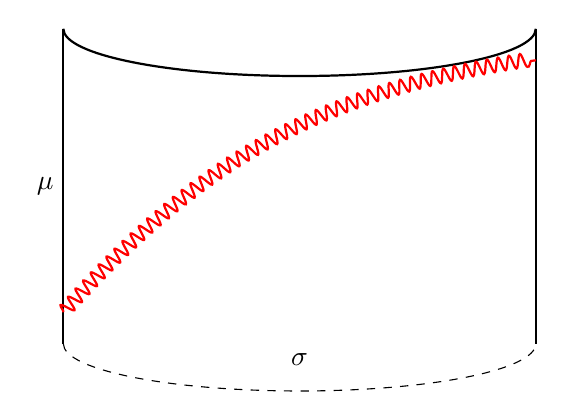
\begin{tikzpicture}[scale=2]
    \draw[thick](0,0)--(0,2);
    \draw[thick](3,0)--(3,2);
    \draw[thick] (0,2) arc(180:360:1.5 and 0.3);
    \draw[dashed](0,0) arc(180:360:1.5 and 0.3);
    \draw[red,thick,decorate,decoration={snake,segment length=4pt}](0,0.2)to[bend left=20](3,1.8);
    \node[left] at(0,1) {$\mu$};
    \node[below] at(1.5,0) {$\sigma$};
 \end{tikzpicture}

\subsection{Overview of Topological Quantum Field Theory} % 3~5 pages
\setstretch{1.2}
\par Following a protracted, intricate, and multi-threaded evolution from the 1930s through the 1970s, quantum field theory culminated in an unprecedentedly and universally successful in applying field theory methods to develop relativistic quantum theory, providing an exceedingly precise picture to describe the electromagnetic force, the weak interaction, and the strong nuclear force down to a remarkably microscopic scale. Via the key theoretical advances of renormalization and gauge field theory during the 1940s to 1960s, the theoretical framework of standard model was yielded, which consists of QED (in the late 1940s), the Glashow-Weinberg-Salam Theory (in the 1960s), and QCD (in the 1970s). Despite its tremendous success in describing the other fundamental interactions, the framework of quantum field theory encountered profound and seemingly insurmountable obstacles in the quantization of gravity. At the Planck length, the gravitational interaction becomes overwhelmingly significant and could no longer be ignored. Since all models in quantum field theory depend on a specific and fixed spacetime background--the Minkowski spacetime, the violent fluctuations of spacetime at such a tiny scale ($10^{-35}$m) obscure many foundational concepts in quantum field theory, and lead to severe deviations in theoretical predictions. These failures imply that QFT is only a theory emerging as a limiting case at a scale where the gravity is negligible; and the resolution of these difficulties seems impossible to be found in quantum field theory itself at all\cite{gross1999}.
\par
\subsection{Historical Background of Chern-Simons Theory} % 2~3 pages